\documentclass{report}


\usepackage{alltt}
\usepackage{graphicx}
\usepackage{color}
\usepackage[small,bf]{caption}
\usepackage{listings}
\usepackage{cite}
\usepackage{url}

\lstdefinelanguage{EzQL}
{
  morekeywords=[1]{from, select, where, group, by, in, hour, min,
    class, end, min, and},
  morekeywords=[2]{max, sumIntervals, avg, @createFrom,
    @hasMany, @belongsTo, sumIntervalsWhereValueIs,
    lengthOfMaxIntervalWhereValueIs},
  sensitive=false,
  morecomment=[l]{\#},
  morestring=[b]",
}

\lstdefinelanguage{CCL}
{
  morekeywords=[1]{dummy, from, select, where, group, by, create, input,
    stream, schema, string, integer, as, window, insert, removed, rows,
  keep, seconds, into, float, last, per, outer, join, boolean,
  if, then, else, end, dummy, ON, left, right, interval, timestamp,
  full, local, and, hours, minutes, dummy}
  morekeywords=[2]{dummy, max, coalesce, now, avg, dummy},
  sensitive=false,
  morecomment=[l]{--},
  morestring=[b]",
}

\lstdefinelanguage{Oracle}
{
  morekeywords={dummy, on, if, then, and, dummy}
  sensitive=false,
  morecomment=[l]{--},
  morestring=[b]",
}


\lstdefinelanguage{MonitorScript}
{
  morekeywords=[1]{dummy, monitor, dictionary, string, int, action, on, all,
    route, if, then, dummy}
  morekeywords=[2]{},
  sensitive=false,
  morecomment=[l]{//},
  morestring=[b]",
}



\definecolor{light-gray}{gray}{0.97}
\definecolor{dark-gray}{gray}{0.50}

\begin{document}
\title{EzQL: A new language for Event Stream Processing}
\author{Lu\'{\i}s Pureza}

\maketitle

\tableofcontents

\addtolength{\parskip}{\baselineskip}
\chapter{Introduction}
\label{chap:introduction}

Technology developments and its widespread adoption over the last
decades have significantly increased the demand for information
processing systems. Not only do we now need to process larger amounts
of information coming from everywhere, we must do it faster as
well. For some companies, obtaining results a few milliseconds earlier
may be a significant advantage over the competition. For others,
however, reacting immediately is of critical importance, as it
happens, for example, in the case of security breaches or nuclear
power plant malfunctions.

One particular class of applications, now referred to as Event Stream
Processing (ESP), has been the subject of much attention over the last
few years due to the potential it presents to solve many real-world
problems. ESP applications are characterized by dealing with a
possible infinite amount of data constantly flowing in to be processed
as fast as possible to continuously produce new and updated results
that may themselves be used to justify new decisions. It turns out
that many applications fit naturally in this model: financial
analysis, health-care monitoring, network intrusion detection,
personnel and product tracking through RFID devices, business
monitoring and many more.

Due to the inability of current technology to satisfy the increasing
demands from all these markets, computer scientists developed the
first Data Stream Management Systems (DSMS) \cite{stream}
\cite{aurora} \cite{telegraphcq}. Coming mostly from the database
community, these researchers intended to build a generic engine that
abstracted away all the low level details of managing streams of data
in high demanding scenarios, while retaining much of the querying
capabilities of regular Database Management Systems (DBMS), so that
they could be easily adapted to a multitude of domains. It's no
surprise then, that the first DSMSs inherited a SQL dialect with some
new extensions. Aurora \cite{aurora}, with its boxes and arrows
graphical queries was the exception, but the operators it provided
still took inspiration from SQL. Later, when the first DSMS hit the
market, some emphasis was put on end-user interaction and some
applications began to include rule-based systems that allow the
developer to specify how he wants to react to events using Event
Condition Action (ECA) rules, a concept developed in the context of
active databases \cite{adbms-manifesto}. At the same time, DSMS began
to incorporate features from Complex Event Processing (CEP) systems,
that allowed the user to detect complex patterns and correlations
among the input streams of data. This required adding new constructs
into the query language. Recently, some companies unhappy with
declarative, SQL-like languages (see, for example,
\cite{sql-impendance-mismatch:post} or \cite{flexstreams-whitepaper}),
began to support procedural languages, more familiar to C and Java
programmers. Nowadays, each product includes its own flavor of a
SQL-like language with its own unique and esoteric extensions, or a
rule-based language, or a procedural language, or any combination of
these three. Besides the obvious issue created by the lack of a
standard, all this variety demonstrates that DSMS applications have
their own needs and a satisfactory end-user query language for them is
yet to be found.

To make matters worse, the semantics on many of these products
disagree in fundamental ways. In \cite{towards_stream_sql_standard},
researchers analyzed how two of the most prominent products from
Oracle and StreamBase reacted in the presence of simultaneous
events. Surprisingly, they found that in some scenarios, not only do
their results diverge between them, but they also differ from the
expected answer. Furthermore, they concluded that this disparity may
be blamed on the semantics employed by each product. It also happens
that many products consistently implement semantics that, despite
working correcly for most problems, turn out to be innapropriate for
others, making some queries difficult, if not impossible, to
write. Will will analyze a few examples in chapter
\ref{chap:simple-questions-complex-answers}.

Nonetheless, more and more organizations are adopting DSMS and relying
on them to process data coming from everywhere, including core
business processes. As a consequence, ESP applications tend to grow
and become more complex. However, it is our opinion that languages
available in currently existing products are not prepared to support
such large applications because they force developers to think in
terms of low-level abstractions, resulting in programs that are
difficult to write and worse to understand. The purpose of this
document is to highlight these problems with concrete examples and
then propose a new query language for ESP systems. This language
provides a set of powerful constructs that exploit new semantics,
allowing it to solve some new ESP problems while keeping the ability
to handle all others, sometimes in better ways.

The rest of this thesis is organized as follows:

\begin{itemize}
\item In chapter \ref{chap:soa}, we will discuss the state-of-the-art
  pertaining to ESP languages;
\item Chapter \ref{chap:simple-questions-complex-answers} expands on
  the previous paragraphs to show a few problems where currently
  available languages show some limitations. We will also discuss how
  they could be fixed;
\item Our proposal --- EzQL ---, will then be introduced in chapter
  \ref{chap:ezql};
\item Further work and planning for the next semester will be the
  topic of chapter \ref{chap:future-work};
\item Finally, chapter \ref{chap:conclusion} concludes this document.
\end{itemize}

\chapter{State-of-the-art}
\label{chap:soa}

This chapter will begin by analyzing SQL dialects present in some
industry products for event processing --- Coral8 \cite{coral8:www},
StreamBase \cite{streambase:www} and Esper \cite{esper:www}. As far as
we know, there isn't any ESP language being actively researched,
although there are efforts to provide more powerful languages to
detect complex patterns of events, such as SASE+ \cite{SASE+}. Pattern
detection is outside the scope of this thesis, because we are
interested in processing events, not detecting them. It should be
noted, however, that these two kinds of languages --- one for
processing and another for detecting ---, are more or less orthogonal
to each other and may be integrated with some work. The document
proceeds with StreamBase EventFlow --- a method for creating queries
visually through a boxes and arrows interface. Despite not involving
programming languages, it's important to study these alternatives
because, after all, they're trying to address the same problem. Next
comes Oracle Rules Manager with its rule-based paradigm for complex
event processing. Finally, we will conclude this chapter analyzing
MonitorScript, a procedural language developed by Progress Apama with
the intention of overcoming the limitations imposed by SQL-like
languages.

\section{SQL-based languages}
\label{sec:sql}

The most popular way of writing queries is through a declarative,
SQL-based language. Products adopting this solution include Coral8
\cite{coral8:www}, StreamBase \cite{streambase:www} and Esper
\cite{esper:www}. As explained in the introduction, this comes as a
result of all the effort the database community has put into creating
the first ESP engines. Currently there is no standard for a query
language designed specifically for these applications which means each
vendor has their own. Fortunately, they're all very similar. The
simplest things can be done exactly as in regular SQL:

\lstset{
  language=CCL,
  columns=fullflexible,
  basicstyle=\tt,
  keywordstyle=[1]\bf,
  keywordstyle=[2]\it,
}

\begin{lstlisting}
  insert into PriceACME
  select *
  from   StockTrades
  where  symbol = 'ACME'
\end{lstlisting}

% TODO: s/MSFT/ACME

This query looks for tuples where the field \verb=symbol= equals
``ACME'' arriving at the stream \verb=StockTrades= and adds them to
the \verb=PriceACME= stream. It's just a simple filter that separates
ACME events from the others.

One feature that assumes particular importance in the context of ESP
is the concept of window. Windows allow developers to consider only a
continuous section of a stream and make computations over it. In
particular, it becomes possible, for example, to calculate the most
expensive order among the last million, or the average of ACME's stock
prices over the last 3 hours, as the following example shows:

\begin{lstlisting}
  insert into AvgPriceACME
  select avg(price)
  from   StockTrades keep 3 hours
  where  symbol = 'ACME'
\end{lstlisting}

More advanced windows allow the developer to retain, for example, the
10 largest updates based on their price, the 10 last updates per
company or simply to keep everything.

The window defined in the previous example is a \emph{sliding}
window. Sliding, in this context, refers to how and when the elements
in the window expire. In these kinds of windows, tuples are removed
from the window as they become too old or new tuples arrive. An
alternative is \emph{jumping} windows, where tuples are appended to
the window and then, when the oldest element was supposed to be
removed, all of them expire at the same time, the window becomes empty
and the cycle begins all over again. This way, it's possible to find
out the largest price attained by ACME stocks over the last hour, the
hour before and so on.

All the examples in this section were written in Coral8 Continuous
Computation Language (CCL) \cite{coral8-ccl:www}. Nonetheless, all the
other systems in this section provide similar features albeit with
different syntax. In fact, there have been talks about creating a
standard language lately, an idea that was met with some skepticism by
some vendors and users that don't like SQL anyway and opted for other
approaches \cite{sql-impendance-mismatch:post}.

With the undeniable increasing relevance of ESP and the predominance
of SQL-based languages in currently-available products, it is
important to analyze the limitations of these languages. After all, it
doesn't make sense to build yet another programming language if the
existing ones are good enough. This will be the topic of the next
chapter.

\section{Building queries visually with StreamBase's EventFlow}
\label{sec:eventflow}

StreamBase employs an alternative, more user-friendly, way of building
queries. Instead of writing code, the user can design queries
visually, by arranging boxes in a canvas and connecting them with
arrows. Boxes represent operators that receive data coming from other
operators or directly from the input streams, process the data
according to its semantics and send the results to be handled by other
operators, or to the world as the output of the whole operation. An
example is shown in figure \ref{fig:eventflow-sample}.

\begin{figure}[htbp]
  \centering
  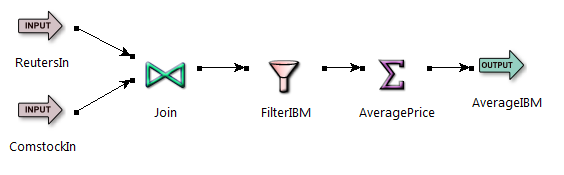
\includegraphics[width=\textwidth]{eventflow.png}
  \caption{This diagram represents a simple query where two streams
    are joined, non IBM tuples are filtered-out, and then the average
    of IBM stock prices over the last 5 minutes is sent to the
    output.}
  \label{fig:eventflow-sample}
\end{figure}

Some of the most important operators are:

\begin{description}
\item [Aggregate] Computes aggregate operations over windows of
  tuples. Supports the option to partition tuples into sets and then
  apply the aggregation over each individual set, much like a SQL
  GROUP BY statement;
\item [Filter] Discards some tuples from the input stream based on a
  predicate. Performs the same function as a SQL WHERE statement;
\item [Gather] Receives tuples from two or more streams and
  concatenates those with the same key. The resulting tuple values may
  be direct copies from the original tuples or the result of applying
  some expression to these;
\item [Join] Similar to SQL joins, this operator pairs tuples coming
  from two streams that match a given condition and outputs a new
  tuple whose fields may be specified by the user. In general, joining
  two infinite streams may require keeping all tuples from both
  streams in memory. To avoid problems later on, the user must specify
  timing constraints regarding matching tuples saying, for example,
  that they must arrive withing 60 seconds of each other;
\item [Map] Similar to the first part of a SELECT statement, this
  operator transforms a tuple --- possibly discarding or adding new
  fields along the way ---, and sends it downstream;
\item [Pattern] Instructs the engine to look for complex events. This
  is a feature borrowed from Complex Event Processing and will be
  discussed below;
\item [Union] Acts as a multiplexer, connecting many input streams to
  a single output stream, to where all tuples are sent. Similar to the
  SQL UNION statement.
\end{description}

It's clear that most of these operators have SQL counterparts. There
are a few things that can be done in EventFlow but not in StreamSQL
(see the online documentation at \cite{eventflow2streamsql}), but
they're just small details, nothing that changes the developer's way
of thinking. It's then mostly a matter of taste --- not power ---, to
choose between StreamSQL and EventFlow.

\section{Oracle rules}
\label{sec:orm}

Oracle Rules Manager (ORM) \cite{orm:www} embraces a completely
different paradigm. Instead of writing queries, the user creates rules
that are made of three parts. The first, the event type, instructs the
system to trigger the rule only when an event of that type occurs. The
second, the condition, is a predicate that is compared against the
event. If they match, the third part, the action --- a PL/SQL
procedure ---, is executed.

Conceptually, a rule has the following format:

\lstset{
  language=Oracle,
  columns=fullflexible,
  basicstyle=\tt,
  keywordstyle=\bf,
}


\begin{lstlisting}
  on   <event>
  if   <condition>
  then <action>
\end{lstlisting}

The following example shows a simple rule:

\begin{lstlisting}
  on   StockTick(symbol, price)
  if   symbol = 'MSFT' and price > 100
  then buyStocks(symbol)
\end{lstlisting}

The event shown above represents a stock update received from some
external source. These are the simplest kind of events, also called
\emph{primitive} events. ORM also supports \emph{composite} events
that are defined as combinations of other events. For example, it is
possible to define a composite event that occurs when Microsoft shares
drop by 10\% and, less than 5 minutes later, IBM shares gain 2\%. To
be more specific, the following types of combinations are supported:
\begin{description}
\item [Sequencing] Specifies the order between events, i.e., event A
  must occur before event B;
\item [Negation] Checks for the non-occurrence of some event. Useful
  to raise exceptions when business rules are violated;
\item [Set semantics] Allows combining events with the AND operator to
  specify that all of them must occur for the composite event to occur
  as well;
\item [Any N] Checks for the occurrence of at least N children events;
\item [Collection] Combines a set of primitive events based on some
  common properties. Could be used, for example, to detect all
  costumers who withdrew more than \$1000 from their bank accounts
  during the past 24h.
\end{description}

ORM comes with a GUI utility to simplify the rules creation
process. This is necessary because creating a rule the hard way is a
daunting task that involves writing SQL queries containing XML blocks
containing SQL snippets inside. Still, there are situations when one
needs to avoid these utilities and work with real code, situations
where a simpler configuration process would be desirable.

The biggest disadvantage of rule-based languages comes from the
paradigm itself. While they may be effective for detecting complex
patterns of events, they are not so good when it comes to actually
processing the data. Built-in combinators provide some aggregation
functions, but these will seem basic for companies in need to
implement proprietary analysis algorithms. Also, PL/SQL is arguably
not a language suited for complex application development.

One other issue that plagues these systems is the difficulty to reason
about their runtime behavior. As the number and complexity of rules
increases, an event may trigger more than one rule and these rules may
themselves trigger other rules, resulting in a cascading process that
may never end. This behavior makes the applications more difficult to
understand, to the point where even adding or removing a simple rule
may have unpredictable effects. These kinds of non-linear interactions
are discouraged by Software Engineering best-practices and thus, the
decision to use rule-based systems for building large applications
must be carefully pondered. To be fair, Oracle Rules Manager provides
constructs to deal with simultaneous triggering rules, but the problem
doesn't go away: only now the developers will be to blame when things
go wrong.

\section{Apama's MonitorScript}

When ESP solutions left the academia to meet the real world, many
users argued that SQL was ill-suited for many information processing
tasks. MonitorScript (MS) is Apama's response to these complains.

Deriving from the procedural family of programming languages, MS
programs look a lot like Java programs. However, the most important
and unique feature it includes is the process model based on having
many little \emph{processes} that execute in parallel and communicate
with each other through messages. In MS, these entities are called
\emph{monitors}. A monitor is an event processing agent that basically
sets up an arbitrary number of \emph{listeners} that await for the
occurrence of events. When one matching event arrives, monitors
process it. Monitors can also send events to each other, through the
\emph{route} statement.

Last but not least, monitors can have state. This means that instead
of writing a SQL query to capture the state of the system, MS updates
the state incrementally as the computation moves forward. The downside
is that, for simple things, SQL queries will definitely be easier to
understand, because a SQL query \emph{is} its intention while, in a
procedural program, the big picture is not always that clear.

To get a feeling for the language, here is a small MonitorScript
snippet:

\lstset{
  language=MonitorScript,
  columns=fullflexible,
  basicstyle=\tt,
  keywordstyle=[1]\bf,
  keywordstyle=[2]\it,
}


\begin{lstlisting}
monitor ProcessMarket {
    // Keep the last price per company
    dictionary <string, int> lastPerCompany;

    action onload {
        Tick tick;
        on all Tick(): tick {
           processTick(tick);
        }

        on all PriceRequest(): ev {
            processPriceRequest(ev);
        }
    }

    action processTick(Tick tick) {
        lastPerCompany[tick.sym] := tick.price;
        route TickAck(tick.sym);
    }

    action processPriceRequest(PriceRequest ev) {
        if (lastPerCompany.hasKey(ev.sym)) then {
            route PriceReply(ev.sym, lastPerCompany[ev.sym]);
        }
    }
}
\end{lstlisting}

This listing declares one monitor (\verb=ProcessMarket=), that waits
for \verb=Tick= and \verb=LastPriceRequest= events. When it receives a
new \verb=Tick= update, it keeps the price reported in a dictionary,
indexed by the company's symbol and replies with a \verb=TickAck=
message. When it receives a \verb=PriceRequest=, it fetches the last
price from the dictionary and sends a \verb=PriceReply= message.

Note the need to create request, reply and acknowledgement messages
when what one really wants to do is to perform a method invocation
between different monitors. Indeed, the runtime system could provide
some kind of remote procedure call mechanism and handle the low-level
details by itself.

MS and SQL are at opposite ends of the programming language
spectrum. While is simplifies a lot of tasks that don't naturally fit
into SQL, MS also looses all the querying capabilities that made SQL
and its derivatives popular for data processing.

\chapter{Simple questions, complex answers}
\label{chap:simple-questions-complex-answers}

In this chapter we are going to discuss some simple queries that are
very complex to express using existing SQL dialects for ESP
systems. We will try to understand the reasons for this difficulty and
propose solutions to eliminate it.

\section{Events are from Mars, state is from Venus}
\label{sec:acme-problem}

% TODO spell checker

In the context of ESP applications, events are always discrete and
stateless entities. Discrete because they have a well defined position
in time, and stateless because the information an event carries
becomes invalid outside that position. This works for many scenarios
that are discrete by nature --- earthquake reports, orders placed in
an online store, heart beats or even noise readings sampled
periodically, just to name a few. However, some systems are truly
continuous and the values reported by an event influence what we know
about the system and what we can conclude about its state. Examples
include price change reports, where we know that the price of a
product will remain the same until a later event signals a change,
temperature readings by a smart sensor that issues reports only when
the temperature differs by 0.1 degrees from the one in the previous
notification, or a goal scored in a football match that updates its
result until another goal is scored or the match ends. Unfortunately,
the semantics employed by ESP systems don't work so well in these
cases.

To see why, let's begin with a small example. Suppose we build an ESP
application to monitor noise-levels in a street, measured by a sensor
every 10 minutes. This application receives the following two events
and no others:

\begin{tabular}{ |l|r| }
  \hline
  Timestamp & Noise (dB) \\
  \hline
  11:00 am & 70 \\
  11:10 am & 50 \\
  \hline
\end{tabular}

Suppose further, that our application is interested only in analyzing
the last 20 minutes of data and, to achieve that, uses a regular
temporal sliding window like the ones discussed in section
\ref{sec:sql}. Figure [something] shows the contents of this window
between 11:00 am and 11:30 am.

% TODO Figure
%
% Before 11:00 -> empty
% 11:00 -> 70
% 11:10 -> 50, 70
% 11:20 -> 50
% 11:30 -> empty

By querying this window, we are now able to answer a few
questions. For example, at 11:10, the loudest reading registered
during the past 20 minutes was 70 dB, while 10 minutes later the
first event expires and the answer becomes 50 dB. Note that you cannot
ask for the loudest moment in the last 20 minutes, because a noisy
ambulance may have passed while the sensor was idle. That is, you
cannot assume anything in the time that goes from one event to
another. However, given the data that is available, the application
returns the correct answer.

This application is so successful that we are asked to adapt it to
monitor the stock market. Our clients are investors who want to be
able to make good decisions as quickly as possible and, to do so, our
application must handle events informing about every single
transaction. Suppose the application is deployed and receives the same
two events from the previous example, where instead of representing
noise-levels, they now refer to the value of ACME stock actions. Using
the same 20 minutes window, we may try to compute the highest price
attained by ACME during this period. At 11:10 am, the application will
return \$70, while at 11:20 am the answer will change to \$50, just
like in the previous example. However, this answer is known to be
wrong because the price remained at \$70 until 11:10 am. Despite using
the same input data, posing the same question and obtaining the same
two results, one was correct while the other was wrong.

The central difference between these two examples, pertains to what
can be assumed between events. There are three different cases:

\begin{itemize}
\item Between events the value is undefined. This is what happens when
  the value is discrete by nature --- the sender of a network packet
  is undefined when there is no network traffic ---, or when the event
  generator is sampling a continuous entity, like the noise sensor of
  the first example. We will refer to this as the \emph{pulse}
  semantics;
\item The value remains constant until the next event modifies
  it. This is valid if the value represents a new state, like the
  price of ACME stock actions, that remains the same between two
  updates. As such, we will call this the \emph{state-changes}
  semantics. Some continuous distributions that are known to be smooth
  may also be modeled under these semantics. For example, temperature
  may be assumed to remain constant between two updates, unless sudden
  variations not reported by the sensors are problematic;
\item In some rare cases, the value between events may be approximated
  by a well known mathematical function.
\end{itemize}

Existing languages adopted the pulse semantics by design. This is a
natural choice if we consider events as isolated occurences. However,
if events represent changes in state, these languages will disappoint
because the developer has to manage this state manually. This can be
seen in Appendix \ref{sec:acme-problem-solution}, where a solution to
the ACME stocks problem, implemented in Coral8 CCL, is shown. The
algorithm creates two windows: the 20 minutes window and another
window that will contain the newest event older than 20 minutes (i.e.,
the event that most recently expired from the 20 minutes
window). Then, we perform a \verb=full outer join= between both
windows (\verb=union= would be more appropriate, but Coral8 doesn't
support it) and calculate the maximum price in either of them. As you
can see, this solution is quite verbose, which would be OK if only
there weren't so many situations like this, where the values are
continuous and must be handled with special care.

A slightly modified version of the ACME problem was posed on an online
community where researchers and vendors participate
\cite{simple-problem} \cite{simple-problem2}. It generated a lengthy
(more than 60 messages), interesting and sometimes funny
debate. Several vendors replied --- including Oracle, Aleri, Coral8
and Esper ---, and tried to find a good solution using their
products. In our opinion, they failed because their solutions were
verbose (like the Coral8 one above), inneficient or wrong. In the end,
some participants concluded this was not an event processing problem
anyway because it envolves state and tried to dismiss it as
irrelevant, while others argued that queries like these show up every
day and if ESP engines can't solve them, their usefulness is reduced.

We agree that existing ESP engines shouldn't be applied to problems
like these, not because they don't matter, but because these engines
were not prepared to solve them --- even if they are able to do so
with more or less trouble. Instead, we believe these problems call for
a new language, encompassing both pulse and state-changes semantics,
that provides first-class constructs to deal with them.

% TODO Remove this

\begin{figure}[htbp]
  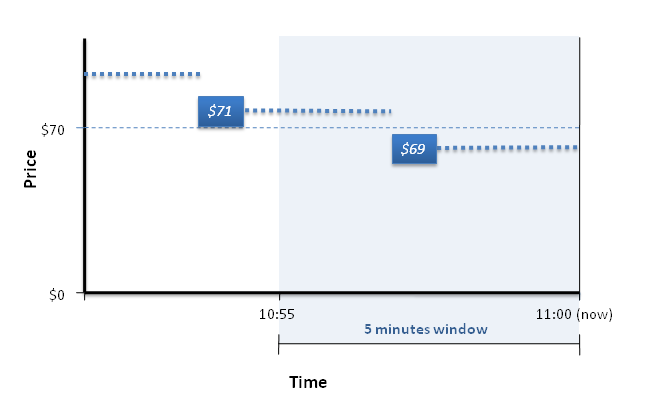
\includegraphics[width=\textwidth]{outside-window.png}
  \caption{Evolution of ACME stock prices in the scenario described in
    the text. Values in blue boxes represent the two events received
    at 10:54 and 10:56. As you can see, the first event lies outside
    the 5 minutes window and thus, will be ignored by the system. The
    dotted blue lines illustrate the fact that prices remain constant
    until the next update, an assumption made by humans that the
    system is unaware of.}
  \label{fig:outside-window}
\end{figure}


\section{Spoiled products detection a.k.a. The ``too muggy'' query}
\label{sec:spoiled-products}

% TODO: Refer that we assume temperature remains constant between
% updates, because the sensor is prepared, blah blah

Another class of problems that are reasonable in the context of ESP
systems but are difficult to solve by current systems are those where
the developer needs to know for how long was a certain condition true
(or false). For example, imagine the following scenario, attributed to
Andrew Witkowski from Oracle: a factory has three rooms, every room
has at least one humidity sensor and one temperature
sensor. Furthermore, products contain a RFID tag that is read by RFID
sensors placed at the entrance and exit of each room. All these
sensors send their readings to a DSMS that needs to answer the
following question: ``Which products stayed more than 10 minutes
(overall, not consecutive) at more than 20 $^{\circ}$C and 80\% of
humidity?''. These products are spoiled and mustn't be sold.

A solution for a simplification of this problem, written in Coral8
CCL, is shown in Appendix \ref{sec:spoiled-products-solution}. This
solution does not take humidity into consideration and assumes there
is only one sensor per room. The algorithm is simple: for each
product, we keep one counter with the time the product spent above 20
degrees, as well as the timestamp for when this counter was last
updated. When a product leaves a room, we update its counter if the
temperature in the previous room was higher than 20, and set the last
updated timestamp to the current time, given by the \verb=now()=
function. When the temperature changes, we do the same thing for all
products in that room.

This solution is quite big as it is and it still doesn't solve the
orignal problem. One may argue that this is a difficult problem and
the solution can't be simple anyway. Nonetheless, it is a good
exercise to analyze this piece of code to see what's wrong with it.

Let's begin by thinking about what would have to be modified to
support humidity. Naturally, we would have to create a new stream ---
\verb=hum_readings= --- that receives humidity readings from
sensors. Then, it would make sense to create a window to keep the last
humidity reading per room, analogous to the \verb=RoomTemperature=
window for temperatures. When the humidity changes, we need to
generate new events with the identifier of the room and its old
humidity, just like we do now when a product switches rooms or when
the temperature changes. When an event arrives on this stream, we
check if the previous humidity was greater than 80\% and if the
current temperature is above 20 degrees. If both conditions hold, we
may finally proceed to update the product's counter as well as its
last updated timestamp. Unfortunately, we are not done yet: it is also
necessary to modify the other queries that are triggered when the
temperature changes or when the product switches rooms, to take the
current humidity level into consideration. Thus, adding new sensors
implies not only writing new queries, but also modifying existing
ones. Clearly, this approach does not scale\footnote{``scale'' here
  refers to the source code, not to the performance of the solution.}
as extensive rewrites are necessary everytime the requirements are
modified. Software engineering best-practices dictate that, if
something like this happens, then the code is not modular enough or is
using the wrong abstractions.

The solution for this problem implemented in the appendix shows some
of these symptoms. There, besides the two input streams and the window
with the counter per product, we create two other windows and two
temporary streams. The windows contain the current and previous
temperatures of each room and the current and previous room for each
product. Thus, these windows are used to maintain the state of the
system. To support humidity, we would need a third window to maintain
the current and previous humidity level for each room. Note how
information (temperature and humidity) for a given entity (the room)
becomes scattered across several windows. To correlate temperature
with humidity, one would need to join these windows and then group by
the room's id. Years of thinking in terms of objects and programming
using the object-oriented paradigm, indicate that this query would be
greatly simplified if there was some way to define \verb=Room= objects
with properties like \verb=currentTemperature= or
\verb=currentHumidity=, and use these objects in queries, just like
regular events. Moreover, one could instruct the system to create the
objects and manage their attributes automatically, by looking at the
right events. We could take this one step further by supporting
relationships between objects, akin to what Object-Relational Mapping
(O/RM) tools like Hibernate \cite{hibernate:www}, do for regular
databases. This way, each \verb=Room= object would possess a list with
its \verb=Product=s and each \verb=Product= would include a reference
to the \verb=Room= where it is at. With these changes, finding the
current temperature of the room where a product is would be as simple
as typing \verb=product.room.currentTemperature=.

As for the two temporary streams, their events are created when the
products switch rooms or when the temperature of a room changes, and
contain the previous room id or the previous temperature. These
streams are not strictly necessary as their code could be directly
inserted into the \verb=FROM= clause of the queries that use
them. However, this would not be a good idea as it would quickly
result in unreadable code. To avoid creating big and complex queries,
developers partition them into smaller ones connected by temporary
streams. Thus, streams end up being used as variables to store the
intermediate results of computations. But streams aren't a suitable
replacement for all kinds of variables. In procedural programming
languages, programmers can choose among primitive variables (int,
float, string, \dots), arrays, dictionaries, lists, sets and, why not,
objects. Certainly, streams and windows alone could be used to
simulate all these kinds of constructs, but they're just not the right
tool for \emph{every} job.


\section{What was the $<$result$>$ while $<$condition$>$ hold?}
\label{sec:result-while}

Suppose that ACME actions were worth more than \$70 during some
interval and you want to know what was the average of their price
during that interval. Solving this problem using current technology is
not so difficult. Most ESP products include some kind of event
detection feature that allows the search for patterns of events. To
obtain an answer, we could find the event where ACME stocks passed the
\$70 mark, then find all the events where the price stayed above that
threshold and finally, find the event where they descended below
\$70. With all these events, we could then proceed to calculate the
average price.

There are two problems with this approach. The first is that the
detection of the boundaries of this interval may itself involve the
detection of another complex pattern. For example, to discover the
event where the price rose above \$70, one needs to compare some event
with the one that preceded it. The second problem is that these
complex event detection features work by first detecting the pattern
and then processing it. Thus, while the price remains above \$70, the
engine keeps all the events in memory and only when the price goes
below that mark will it proceed to calculating the average. This is
suboptimal, because the engine could keep a temporary sum of the
prices and a temporary count of the number of events received. These
two numbers are enough to generate the average and thus, the events
themselves could be discarded immediately.

In the previous section \ref{sec:spoiled-products} we concluded that
the evolution of stock prices could be seen as a continuous
function. Then, conceptually, solving this problem should be as easy
as writing a continuous query that calculates the average \emph{while}
the price is greater than \$70.


\section{Variable windows}

We've seen before that ESP systems provide many windowing facilities
on top of regular SQL -- sliding windows, jumping windows, windows per
groups, etc. However, all these windows share a common limitation:
their sizes are fixed. Suppose you have a new stream whose events
represent requests to calculate the average price of the last N stock
updates for some company. Usually, this would be solved by creating a
window that keeps the last N events for that company. Imagine,
however, that N is a field of the request --- i.e., the client decides
how many events to use in the calculation ---, with the restriction
that it must be smaller than some arbitrary number (otherwise it would
be necessary to keep everything in memory). Unfortunately, we don't
know of any way to solve this using SQL dialects in existing products,
because its not possible to create variable-sized windows even if they
are contained inside a bigger window.

Some may argue that this is not event processing at all because it
involves requests that are better handled by a traditional
DBMS. Still, these scenarios may be more frequent than one thinks and
it doesn't seem like it's complex to implement anyway.

\section{A different perspective}

In this chapter we have shown that there are problems where existing
languages perform poorly. We believe this happens because these
languages work at a very low level which forbids the developer to
think in terms of higher abstractions. For example, the sliding window
discussed in section \ref{sec:acme-problem} only knows about events and
ignores their meaning. The \verb=JOIN=s and \verb=GROUP BY=s employed
in the resolution of the spoiled products problem are necessary
because there is no way to keep related information together. In
section \ref{sec:result-while} we discussed that, in order to identify
the moment the stock price passes some threshold, it is necessary to
look at past events. Meanwhile, thinking of the evolution of price as
a continuous function would give a much simpler answer.

It's not our purpose to claim that SQL, in general, is not well-suited
for ESP applications. However, we believe that ESP problems have their
own needs that require the availability of new data types, new
operators and different semantics, to the point where the resulting
language can hardly be called a SQL dialect anymore. Still, SQL has
benefits. For simple things, its declarative nature makes it very
expressive. After all, queries represent, almost in English, the
intention of the developer. Also, SQL querying capabilities are very
powerful and excel in many data processing tasks. It is understandable
then, that a new language should take some inspiration from SQL and
borrow some features to provide equally powerful constructs.

\chapter{The EzQL query language}
\label{chap:ezql}

\lstset{
  language=EzQL,
  columns=fullflexible,
  basicstyle=\tt,
  keywordstyle=[1]\bf,
  keywordstyle=[2]\it,
  % frame=leftline,
  % framerule=1pt,
  % rulesep=20pt,
  % backgroundcolor=\color{light-gray},
  % rulecolor=\color{dark-gray}
}

In this chapter we introduce EzQL, our proposal to attack the issues
outlined in the previous chapter. Its main features are:

\begin{itemize}
\item The language integrates both pulse and state-changes semantics,
  discussed in the previous chapter. Thus, \emph{EzQL does not lose
    any hability offered by current systems}\footnote{At least in
    theory. In practice some things may not be implemented due to the
    lack of time.}, while it also adds new capabilities;
\item Includes a simple \emph{object-model} where real-world entities
  can be modeled as objects with properties --- temperature, price or
  speed, for example ---, whose values depend on the values of
  events. For instance, this object-model allows the creation of many
  Room objects each with their own temperature attribute which is
  automatically updated as new sensor readings arrive. Furthermore,
  these objects and the values of their properties define the state of
  the application and this state can be queried just like regular
  events;
\item The object model supports \emph{associations} between objects,
  inspired by Ob\-ject-Relational Mapping (O/RM) tools for
  databases. Thus, it is possible to say, for instance, that a room
  has many products and, correspondingly, that a product belongs to
  one room. Again, these associations may change as new events arrive,
  i.e., a product may leave one room and enter another. Naturally,
  these relationships can also be queried --- one can ask, for
  example, which is the cheapest product inside room A. This type of
  queries can already be written in currently available systems, but
  we will see that they become much simpler in EzQL;
\item EzQL provides some support for \emph{temporal queries}, a common
  class of queries in ESP applications that current products don't
  always handle so well, as we have seen. This support integrates with
  the object-model so that one can easily ask, for example, for how
  long was the temperature in some room above 20$^{\circ}$C during the
  last 10 minutes;
\item Combines the \emph{imperative} (C, Java) and the
  \emph{declarative} (SQL) paradigms allowing the developer to query
  data with a SQL-like language or by writing an algorithm, specified
  as a sequence of small steps, for those cases where SQL is not
  appropriate;
\end{itemize}

Before we delve into the language, it's important to mention that, at
this point, the syntax is not yet set in stone. Right now, the
semantics are the most important thing, specially because continuous
queries on streams are conceptually different from the regular
sequential programming we are used to, as we will see. Besides, when
designing a new language, syntax is the easiest thing to change.

\section{Operations on streams}
\label{sec:stream-operations}

To manipulate raw streams of data, EzQL supports the basic constructs
that can be found in other languages. As such, we will discuss these
features very briefly.

Suppose you have a stream called \verb=stocks= that receives events
with two fields --- \verb=:symbol= and \verb=:price= ---, that
receives the following events at the given timestamps:

\begin{tabular}{ |l|l|r| }
  \hline
  Timestamp & \verb=:symbol= & \verb=:price= \\
  \hline
  10:59:59 am & \verb="ACME"= & 50 \\
  11:00:02 am & \verb="ACME"= & 52 \\
  11:00:03 am & \verb="XPTO"= & 70 \\
  11:00:06 am & \verb="XPTO"= & 75 \\
  11:00:07 am & \verb="ACME"= & 50 \\
  \hline
\end{tabular}

You may filter ACME stocks, double their price and store the results
in a new stream by doing:

\begin{lstlisting}
  acme_stocks_2x =
    from ev in stocks
    where ev.symbol == "ACME"
    select { :new_price => ev.price * 2 }
\end{lstlisting}

Three things in this snippet may require further explanation. First,
the portion between \verb={ ... }= creates a new tuple with one field
--- \verb=:new_price= ---, which is equal to the original price times
two.

Second, the seasoned SQL developer may find weird the fact that the
\verb=select= comes after the \verb=from=. The rationale behind this
decision is that variables are declared in the \verb=from= clause
before they are used in the rest of the query. This way, an advanced
editor will be able to assist the developer for example, by showing
the fields of the \verb=ev= event when he types in \verb='ev.'=. Once
again, this is a syntax issue and may be modified if we conclude that
it bothers developers.

Third, we did not specify a timestamp for the new events. This is
because the timestamp is a special field, common to all events, that
is managed by the engine.

After 11:00:07 am, the stream \verb=acme_stocks_2x= will contain the
following events:

\begin{tabular}{ |l|r| }
  \hline
  Timestamp & \verb=:new_price= \\
  \hline
  10:59:59 am & 100 \\
  11:00:02 am & 104 \\
  11:00:07 am & 100 \\
  \hline
\end{tabular}

Notice that \verb=acme_stocks_2x= is an active stream that receives
events and processes them on arrival, as can be seen by comparing the
timestamps in both streams. Thus, if new ACME stock reports arrive
into the \verb=stocks= stream, their price will be doubled and then
sent to the \verb=acme_stocks_2x= stream. This is a very important
point to make: since these queries are continuous --- i.e., they are
always executing ---, results may change as time passes or new events
arrive.

The next example shows a more complicated query that calculates, for
every company, the maximum price of its stocks over the last hour:

\begin{lstlisting}
  max_per_company_1h =
    from ev in stocks[1 hour]
    group by ev.symbol
    select max(ev.price)
\end{lstlisting}

The result of this query is a dictionary that maps company symbols to
their maximum prices. At 11:10:00, for example, this dictionary will
contain:

\begin{tabular}{ |l|c| }
  \hline
  \verb=:symbol= & \verb=max(ev.price)= \\
  \hline
  \verb="ACME"= & 52 \\
  \verb="XPTO"= & 75 \\
  \hline
\end{tabular}

Just like most data types in EzQL, this dictionary will be
automatically updated to reflect the arrival of new events or the
passage of time. For example, if reports from previously unseen
companies arrive, a new entry will be added to the dictionary; and if
ACME stocks rise, their corresponding maximum price will be modified
as well.

Other operations such as joining streams with windows, filtering
groups or sorting windows are also supported, but we won't discuss
them here as they are similar to their counterparts in other
languages. Notice, however, that these operations are enough to
support the pulse semantics introduced in the previous chapter,
allowing EzQL to handle most --- if not all --- problems that existing
products already solve.

\section{Modeling entities with objects}
\label{sec:objects}

In chapter \ref{chap:simple-questions-complex-answers}, we argued that
some queries would become simpler if the developer could model the
state of each entity and the relationships between them using
objects. In this section we will explain how to do this in EzQL using
the spoiled products detection example from section
\ref{sec:spoiled-products}.

Suppose you have three streams:

\begin{itemize}
\item \verb=temp_readings(:room_id, :temperature)= which receives
  temperature readings per room;
\item \verb=hum_readings(:room_id, :humidity)= where humidity readings
  are sent to;
\item and finally, \verb=entries(:room_id, :product_id)= whose events
  are created when a product has entered a room.
\end{itemize}

Defining a class \verb=Room= in EzQL can be done as follows:

\begin{lstlisting}
  # A room is created every time a new room_id is seen in any of
  # these streams
  @createFrom(temp_readings, onNew = :room_id)
  @createFrom(hum_readings,  onNew = :room_id)
  class Room
  end
\end{lstlisting}

This code declares a new class --- \verb=Room= ---, but leaves the
declaration empty. However, is also tags the class with two
\verb=@createFrom= annotations. This signals the ESP engine to
automatically create new \verb=Room= instances when previously unseen
\verb=room_id=s show up in either \verb=temp_readings= or
\verb=hum_readings= streams.

In addition, this annotation adds the stream fields to
the class. This way, every Room instance ends up with three
attributes: \verb=room_id=, \verb=temperature= and
\verb=humidity=. These attributes are automatically filled and updated
by the system as new events arrive, so that the developer doesn't have
to worry with these details. Naturally, the values of these attributes
are independent from object to object. That is, an event with
\verb=room_id= equal to 2 will only affect the \verb=Room= instance
with \verb=room_id= equal to 2 and not the others.

Having set up this apparatus, we can now run the simulation and see
the objects being created for us automatically. All the \verb=Room=
instances are accessible using \verb=Room.all=. In essence, this is a
dictionary that maps object id's (taken from the \verb=:room_id= field
in this case) to the objects themselves. If the stream
\verb=temps_readings= contains:

\begin{tabular}{ |l|l|c| }
  \hline
  Timestamp & \verb=:room_id= & \verb=:temperature= \\
  \hline
  11:00:00 am & \verb="A"= & 20 \\
  11:01:00 am & \verb="B"= & 21 \\
  11:02:00 am & \verb="A"= & 23 \\
  11:03:00 am & \verb="B"= & 22 \\
  \hline
\end{tabular}

and if \verb=hum_readings= receives:

\begin{tabular}{ |l|l|c| }
  \hline
  Timestamp & \verb=:room_id= & \verb=:temperature= \\
  \hline
  11:00:30 am & \verb="B"= & 0.60 \\
  11:01:30 am & \verb="A"= & 0.62 \\
  11:02:30 am & \verb="A"= & 0.61 \\
  11:03:00 am & \verb="B"= & 0.59 \\
  \hline
\end{tabular}

then \verb=Room.all=, if evaluated after 11:03:00 am, will return:

\begin{tabular}{ |l|l| }
  \hline
  Object id & Object \\
  \hline
  \verb="A"= & Room with room\_id = \verb="A"=, temperature = 23, humidity = 0.61 \\
  \verb="B"= & Room with room\_id = \verb="B"=, temperature = 22, humidity = 0.59 \\
  \hline
\end{tabular}

Note that the temperature inside room A is 23 degrees even though the
last update was received at least 1 minute ago. It's like in a regular
OOP programming language: if an attribute isn't modified, it retains
the previous value.

Naturally, we can query these objects as if they were normal streams:

\begin{lstlisting}
  from   room in Room.all
  where  room.humidity > 0.60
  select room.room_id
\end{lstlisting}

This would result in a subset of \verb=Room.all= containing only one
room:

\begin{tabular}{ |l|l| }
  \hline
  Object id & Object \\
  \hline
  \verb="A"= & Room with room\_id = \verb="A"=, temperature = 23, humidity = 0.61 \\
  \hline
\end{tabular}

Individual \verb=Room=s may be accessed by indexing \verb=Room.all=
with the room's id. For instance, evaluating
\verb=Room.all["A"].temperature= would result in 23.

Modeling associations between entities is just as easy. For instance,
to specify the one-to-many relationship between products and rooms you
would just need to add a few annotations to the declarations:

\begin{lstlisting}
  # A room is created every time a new room_id is seen in any of
  # these streams.
  @createFrom(temp_readings, onNew = :room_id)
  @createFrom(hum_readings,  onNew = :room_id)
  @hasMany(:products) # There may be many products inside one room
  class Room
  end

  # A product is created every time a new product_id is seen.
  @createFrom(entries, onNew = :product_id)
  @belongsTo(:room)  # A product is inside one room
  class Product
  end
\end{lstlisting}

The \verb=@hasMany= annotation means that each room may contain an
unbounded number of products. This annotation also adds a list of
\verb=Product= instances to every \verb=Room=. So, if you want to get
the list of products in room A you can do so with:

\begin{lstlisting}
  Room.all["A"].products
\end{lstlisting}

The \verb=@belongsTo= annotation adds the reverse association, i.e.,
it means that every product is inside one room. Moreover, this
annotation also adds an attribute \verb=room= to every
\verb=Product=. Thus, to know in which room is product X one could
write:

\begin{lstlisting}
  Products.all["X"].room
  # or ...
  Products.all["X"].room.room_id  # ... to get just the ID
\end{lstlisting}

And you can find the number of products per room using:

\begin{lstlisting}
  from   room in Room.all
  select { :room_id => room.room_id,
           :product_count => room.products.length }
\end{lstlisting}

In this example, \verb=length= returns the number of elements in a
list.

All these attributes created automatically are managed by the engine
without any additional effort required from the programmer. Thus, when
product X enters room B, its \verb=room= attribute will now point to
room B and the room's \verb=products= list will contain a reference to
product X.

This may seem like a bit of hidden magic at first, but it's really
just a simple convention:

\begin{enumerate}
\item The \verb=:products= parameter to the \verb=@hasMany= annotation
  instructs the engine to create a list of \verb=Product=
  instances. It knows that this list should hold \verb=Product=s,
  because ``product'' is the singular of ``products''. This list will
  be named \verb=products=;
\item On the other hand, the \verb=:room= parameter to the
  \verb=belongsTo= annotation tells the engine to create a field named
  \verb=room= in every product. This field will hold an instance of the
  \verb=Room= class (once again, it finds the class name through the
  parameter);
\item The engine fills the \verb=room= attribute of every product by
  checking its \verb=room_id= field. Remember, this field was created
  automatically by the \verb=@createFrom= annotation. Given the
  identifier of the room, the engine can easily lookup the
  corresponding \verb=Room= instance using the \verb=Room.all=
  dictionary;
\item The \verb=products= list in every \verb=Room= is filled using
  the reverse relationship. That is, the products that belong to room
  ``A'' are those where the condition \verb!room_id == "A"! is true.
\end{enumerate}

\section{Continuous values}
\label{sec:continuous-values}

Just as you may query windows containing old events, you may reference
old attribute values in your queries. For example, you can calculate
the maximum temperature of room A over the last 5 minutes using the
\verb=temperature= attribute from the \verb=Room= class as follows:

\begin{verbatim}
Room.all["A"].temperature[5 min].max()
\end{verbatim}

You could have solved this using standard stream operators presented
in chapter \ref{sec:stream-operations}, without creating objects:

\begin{lstlisting}
  from   ev in temp_readings
  where  ev.room_id == "A"
  select max(ev.temperature)
\end{lstlisting}

Surprisingly though, the results may differ. To see why, note that
this is just another instance of the ACME problem --- ``Were ACME
stocks above \$70 during any moment of the last 5 minutes?'' ---
discussed in section \ref{sec:acme-problem}: the temperature could have
been at its maximum 5 minutes ago\footnote{Once again, we assume
  temperatures remain constant between updates.}, but the notification
for this reading might have happened a little earlier and thus, a
regular sliding window applied to a stream would not consider it when
calculating the maximum.

Objects, on the other hand, behave differently. As mentioned in
section \ref{sec:objects}, an object's attribute retains its value
until a new event changes it. One could plot the evolution of an
attribute over time as a step function that changes when new events
arrive, as figure [something] illustrates for hypothetical values of
the \verb=Room.all["A"].temperature= attribute. As the plot shows, the
temperature is at its maximum when the window opens and keeps its
value until it drops a few minutes later, well inside the 5 minutes
window. Thus, querying the attribute for its maximum value over the
last 5 minutes would consider all the values the attribute possessed
during that time --- even if the corresponding event came earlier ---
and would give the correct result.

[TODO Picture]

This is surprising because objects were introduced with the intention
of simplifying queries. But objects also introduce state and this
seemingly innocuous change has profound implications. In essence,
events are discrete while attributes are continuous --- i.e., their
value is always defined. With objects, writing many state related
queries --- like the one in this example --- becomes easier than using
only regular stream operations.

Just for the sake of completeness, here is the solution to the window
problem written in EzQL:

\begin{lstlisting}
  # Companies are created when new symbols appear
  @createFrom(stocks, onNew = :symbol)
  class Company
  end

  above_70 = Company.all["ACME"].price[5 min].max() > 70
\end{lstlisting}

% TODO: Complete, write this in other places
Notice that, with objects and continuous values, we can now support
the state-changes semantics discussed in chapter
\ref{chap:simple-questions-complex-answers} while retaining support
for pulse semantics by using regular stream operations.

Attributes belong to a broader class of expressions called
\emph{continuous values}, which we may define as expressions whose
past history is well known. This past history includes not only the
past values the expressions evaluated to, but also the time interval
in which they did. Continuous values provide an elegant way to solve
many time related queries, as we will see next.

\subsection{Aggregators over continuous values}

The fact that continuous values retain their previous values allows
one to compute aggregations over those values as we saw
above. However, continuous values hold two dimensions of information:
their previous values and the time intervals for when those values
hold. The traditional aggregations we are used to --- \verb=max=,
\verb=avg= and \verb=sum=, among others ---, only care for the
previous values. But we can exploit the time intervals information to
create and experiment with new kinds of aggregators. For example,
imagine you want to know for how long the temperature was equal to 25
degrees. We could create a \verb=sumIntervalsWhereValueIs= aggregator
that checks the past history of the temperature and sums the intervals
where it was equal to some parameter. Then, answering the question
would be as simple as:

\begin{lstlisting}
  Room.all["A"].temperature.sumIntervalsWhereValueIs(25)
\end{lstlisting}

Or you could find the biggest interval where the temperature was 25
degrees using another aggregator,
\verb=lengthOfMaxIntervalWhereValueIs=:

\begin{lstlisting}
  Room.all["A"].temperature.lengthOfMaxIntervalWhereValueIs(25)
\end{lstlisting}

These aggregators have rather lengthy names and they have a few
limitations. For instance, they only consider intervals with the same
value. What if you need to know for how many minutes was the
temperature above or below a certain threshold?

\subsection{Continuous queries produce continuous values}

Suppose you need to know if the current temperature is above or equal
to 25 degrees:

\begin{lstlisting}
  Room.all["A"].temperature >= 25
\end{lstlisting}

This expression it will return either \verb=true= or \verb=false=. But
what happens if the expression is used as part of a continuous query?
Continuous queries are always running and producing results. Hence,
the query should produce \verb=true= when the temperature reaches 25
degrees and \verb=false= when it descendes below 25. That is, in the
continuous context, the entire expression has a value every time the
continuous attribute, \verb=Room.all["A"].temperature=, is
defined. The following table shows this correspondence for some
possible values of the temperature:

\begin{tabular}{ |l|r|r| }
  \hline
  Time interval & \verb=temperature= & \verb!temperature >= 25! \\
  \hline
  $[$10:50; 10:53) & 25.0 & \verb=true=  \\
  $[$10:53; 10:55) & 24.9 & \verb=false= \\
  $[$10:55; 10:56) & 24.8 & \verb=false= \\
  $[$10:57; 10:59) & 24.9 & \verb=false= \\
  $[$10:59; 11:00) & 25.0 & \verb=true=  \\
  \hline
\end{tabular}

The boolean expression has a current value as well as a collection of
previous values. By definition then, the boolean expression is,
itself, a continuous value. So we can just use new aggregators like
the ones defined in the previous section to perform arbitrary
computations on these values. For example, to sum the time intervals
where the temperature was equal or above 25 degrees, we could use the
\verb=sumIntervals= aggregator, which sums up the intervals where the
value is \verb=true=:

\begin{lstlisting}
  (Room.all["A"].temperature >= 25).sumIntervals()
\end{lstlisting}

This expression would return 4 minutes for the temperature values
presented in the previous table.

Note that to find out for how long the temperature was equal to 25
degrees, you could now write:

\begin{lstlisting}
  (Room.all["A"].temperature == 25).sumIntervals()
\end{lstlisting}

This approach is certainly more understandable (and generic!) than
using the aggregators defined in the previous section.

\subsection{Composite attributes}

Let's go back to the spoiled products detection example from section
\ref{sec:spoiled-products}. Suppose we have the following
sequence of events arriving into the \verb=entries= stream:

\begin{tabular}{ |l|l|c| }
  \hline
  Timestamp & \verb=:product_id= & \verb=:room_id= \\
  \hline
  10:00 am & \verb="X"= & \verb="A"= \\
  10:10 am & \verb="X"= & \verb="B"= \\
  10:17 am & \verb="X"= & \verb="C"= \\
  \hline
\end{tabular}

That is, the product X enters room A at 10 am, 10 minutes later it
enters room B and finally, at 10:17 am it enters room C. After all
these events are received, the attribute
\verb=Product.all["X"].room_id= will be a continuous value with the
following history:

\begin{tabular}{ |l|r| }
  \hline
  Time interval & \verb=Product.all["X"].room_id= \\
  \hline
  $[$10:00; 10:10) & \verb="A"= \\
  $[$10:10; 10:17) & \verb="B"= \\
  $[$10:17;   now) & \verb="C"= \\
  \hline
\end{tabular}

Suppose we enrich our \verb=Product= instances with a temperature
attribute which gets its value from the temperature of the room the
product is in:

% TODO: New lines should come in bold

\begin{lstlisting}
  @createFrom(entries, onNew = :product_id)
  @belongsTo(:room)
  class Product
      # The temperature of a product is the
      # temperature of its room
      temperature = this.room.temperature
  end
\end{lstlisting}

As in Java or C++, \verb=this= is a reference to the current product
whose temperature is being accessed.

Finally, assume the following events are received in the temperature
readings stream --- \verb=temp_readings=:

\begin{tabular}{ |l|l|c| }
  \hline
  Timestamp & \verb=:room_id= & \verb=:temperature= \\
  \hline
  09:50 am & \verb="A"= & 10 \\
  10:09 am & \verb="B"= & 15 \\
  10:16 am & \verb="C"= & 20 \\
  \hline
\end{tabular}

If we correlate \verb=entries= and \verb=temp_readings=, we see that
the temperature in room A was 10 degrees while the product X was
there, the temperature in room B was 15 degrees while the product was
there and finally, the temperature in room C was 20 degrees while the
product was there. Since the temperature of a product was defined as
the temperature of the room the product is in, the \verb=temperature=
attribute for product X will contain the following history:

\begin{tabular}{ |l|r|r| }
  \hline
 Time interval & Product X temperature \\
  \hline
  $[$10:00; 10:10) & 10 \\
  $[$10:10; 10:17) & 15 \\
  $[$10:17;   now) & 20 \\
  \hline
\end{tabular}

Now, you could, for instance, calculate the amount of time the
product's temperature was below 15 degrees with:

\begin{lstlisting}
  (Product.all["X"].temperature < 15).sumIntervals()
\end{lstlisting}

Under the previous values, this expression would return 10 minutes.

Even though the current temperature of the product equals the current
temperature of its room, the history of temperatures of the product
does not equal the history of temperatures of its \emph{current}
room. The engine knows that the product switches rooms and is smart
enough to obtain the temperatures from the correct places. Note that
this behavior is embodied in the semantics of the \verb=.= (dot)
operator used in the definition of the \verb=temperature=
attribute.

\subsection{Aggregators as continuous values}
\label{sec:aggregators-continuous-values}

If you remember from section \ref{sec:stream-operations}, the value of
an aggregator may change in response to a new event or simply as time
passes. Also, aggregators are like attributes in that they retain
their values until one of these conditions make them change. Thus,
like attributes, aggregators may be seen as another kind of continuous
values.

Using the \verb=sumIntervals= aggregator introduced in the previous
section, it is straightforward to find out for how long was the
average above some threshold. Assuming the \verb=acme_stocks= stream
contains the ACME stock data we want to analyze, we could write:

\begin{lstlisting}
  (acme_stocks.avg(:price) > THRESHOLD).sumIntervals()
\end{lstlisting}

% TODO: Solve MACD

We are now in a condition to solve the spoiled products detection of
section \ref{sec:spoiled-products}. The complete solution in EzQL is
transcribed below:

% TODO: Again, bold lines for new stuff

\begin{lstlisting}
  @createFrom(temp_readings, onNew = :room_id)
  @createFrom(hum_readings,  onNew = :room_id)
  @hasMany(:products)
  class Room
  end

  @createFrom(entries, onNew = :product_id)
  @belongsTo(:room)
  class Product
      temperature = this.room.temperature
      humidity    = this.room.humidity
  end

  # Spoiled products spent at least 10 minutes at more than 20
  # degrees and 80% of humidity
  spoiled_products =
    from   prod in Product.all
    where  (prod.temperature > 20 and prod.humidity > 0.80)
             .sumIntervals() >= 10 min
    select prod
\end{lstlisting}

The reader is invited to compare this solution with the one presented
in the appendix \ref{sec:spoiled-products-solution} written in Coral8
CCL. In particular, note how easy it was too include the humidity in
our solution. Note also how the information regarding the status of
each product and each room is now encapsulated inside \verb=Room= and
\verb=Product= objects. Moreover, notice how the \verb=sumIntervals=
aggregator maintains an implicit counter for each product, with the
amount of time the product spent under the given conditions, that we
had to manage manually in the CCL.

\chapter{Future work}
\label{chap:future-work}

% TODO

\chapter{Conclusion}
\label{chap:conclusion}

% TODO

\bibliography{thesis}
\bibliographystyle{plain}


\appendix
\chapter{Solutions to a few problems}

This appendix contains solutions to some of the problems discussed in
chapter \ref{chap:simple-questions-complex-answers}. We can't claim
these are the best solutions nor the smallest, but they shouldn't be
too far away. We added a few comments to help the understanding of the
code.

\section{The ACME problem}
\label{sec:acme-problem-solution}

\lstset{
  language=CCL,
  columns=fullflexible,
  basicstyle=\tt,
  keywordstyle=[1]\bf,
  keywordstyle=[2]\it,
}


\begin{lstlisting}
-- Algorithm:
--
-- Keep two windows: one for the last 20 minutes of data, and another
-- with the newest event that is older than 20 minutes (i.e., the one
-- that expired last from the first window). Then, join both windows
-- (union would be better, but Coral8 doesn't support it) and get
-- the max of prices in any of the two windows.

create input stream StreamIn
schema (
   symbol string,
   price  float
);

-- Keep the events from the last 20 minutes.
create window Last20Mins
schema (
  symbol string,
  price  float
) keep 20 minutes
insert removed rows into Expired;

 -- Insert the events into the window.
insert into Last20Mins
select *
from StreamIn;

-- Keeps the previously expired event from Last20Mins (one per symbol)
create window Expired
schema (
  symbol string,
  price  float
) keep last per symbol;

-- For each symbol, store its max value over the last 20 minutes.
create window Result
schema (
  symbol string,
  result float
) keep last per symbol;

-- Join both windows and get the max of either of them
-- This would be prettier with UNION
--
-- Note: When events expire, this generates two events: one before
--       the expiration and another after.
insert into Result
select L.symbol,
       max(coalesce(max(L.price),0), coalesce(max(E.price),0))
from   Last20Mins as L full outer join Expired as E
         on L.symbol = E.symbol
group by L.symbol;
\end{lstlisting}

\section{The spoiled products problem}
\label{sec:spoiled-products-solution}

This is just a simplification of the original problem. In particular,
it doesn't handle humidity and assumes that rooms have a single
temperature sensor.

\begin{lstlisting}
-- Algorithm:
--
-- - Always maintain an explicit counter per product containing
--   the number of seconds the product spent at > 20 degrees.
--   This counter also contains the time the product was last
--   updated (last_update).
--
-- - When a product switches rooms, if the temperature in the
--   previous room was > 20, add now() + last_update to the
--   counter and replace the previous last_update with now();
--
-- - When the temperature in a room changes, if the previous
--   temperature was > 20, add now() + last_update to the
--   counter and replace the previous last_update with now();
--

create input stream entries
schema (
   product_id string,
   room_id string
);

create input stream temp_readings
schema (
   room_id string,
   temperature integer
);

-- Holds the last two entries per product
create window ProductRoom
schema (
   product_id string,
   room_id string
) keep 2 rows per product_id;

insert into ProductRoom
select *
from entries;

-- Holds the last two temp_readings per room
create window RoomTemperature
schema (
   room_id string,
   temperature integer
) keep 2 rows per room_id;

insert into RoomTemperature
select *
from temp_readings;

create local stream OnExit
schema (
   product_id string,
   old_room_id string
);

-- When a product leaves a room, generate an event containing the
-- product and the old room.
insert into OnExit
select entries.product_id, ProductRoom.room_id
from   entries left outer join ProductRoom
         on entries.product_id = ProductRoom.product_id
where  entries.room_id != ProductRoom.room_id;

create local stream OnTemperatureChange
schema (
   room_id string,
   old_temperature string
);

-- When the temperature changes, generate an event containing the
-- room and the old temperature
insert into OnTemperatureChange
select temp_readings.room_id, RoomTemperature.temperature
from   temp_readings left outer join RoomTemperature
         on temp_readings.room_id = RoomTemperature.room_id
where  temp_readings.temperature != RoomTemperature.temperature;

-- Per each product, maintain a counter with the time the product
-- spent above 20 degrees and the last time this counter was updated
create window ProductTemperatureCounter
schema (
   product_id    string,
   time_above_20 interval,
   last_update   timestamp
) keep last per product_id;

-- Initialize this counter
insert into ProductTemperatureCounter
select product_id, 0 seconds, now()
from entries
where room_id = "A";

-- Every time the product leaves the room, checks if the temperature
-- in the old room was > 20 and updates the counter of that product
insert into ProductTemperatureCounter
select E.product_id,
       if T.temperature > 20
         then time_above_20 + now() - C.last_update
         else time_above_20
       end,
       now()
from  OnExit as E, RoomTemperature as T,
      ProductTemperatureCounter as C
where E.old_room_id = T.room_id
        and E.product_id = C.product_id;

-- Every time the temperature changes, checks if the previous
-- temperature was > 20 and updates the counters of all the products
-- in that room
insert into ProductTemperatureCounter
select R.product_id,
       if T.old_temperature > 20
         then time_above_20 + now() - C.last_update
         else time_above_20
       end,
       now()
from  OnTemperatureChange as T, ProductRoom as R,
      ProductTemperatureCounter as C
where T.room_id = R.room_id
        and R.product_id = C.product_id;
\end{lstlisting}

\end{document}